\documentclass{article}
\usepackage{tcolorbox}
\usepackage{ntheorem}
\usepackage{amsmath}
\usepackage{amssymb}
\usepackage{ulem}
\usepackage{graphicx}
\usepackage{centernot}
\usepackage{tikz}
\usepackage{tabularx}
\usepackage{pgfcore}

\usepackage[margin=1in]{geometry}
\usepackage[parfill]{parskip}

\everymath{\displaystyle}

\makeatletter
\newtheoremstyle{MyNonumberplain}%
  {\item[\theorem@headerfont\hskip\labelsep ##1\theorem@separator]}%
  {\item[\theorem@headerfont\hskip\labelsep ##3\theorem@separator]}%
\makeatother
\theoremstyle{MyNonumberplain}
\theorembodyfont{\upshape}

\theoremstyle{break}
\newtheorem*{proof}{Proof. }

\newcommand{\R}{\mathbb{R}}
\newcommand{\Q}{\mathbb{Q}}
\newcommand{\Z}{\mathbb{Z}}
\newcommand{\N}{\mathbb{N}}
\newcommand{\C}{\mathbb{C}}
\newcommand{\cyclic}[1]{\langle #1 \rangle}
\newcommand{\nline}{\begin{tabular}{ll}&\\\end{tabular}}
\newcommand{\nin}{\not\in}
\newcommand{\p}{\phi}
\newcommand{\infixor}{\text{ or }}
\newcommand{\infixand}{\text{ and }}
\newcommand{\ord}[1]{\text{ord}(#1)}


\newtcolorbox{prfbox}{colback=gray!10,colframe=black!70,boxrule=0pt,arc=0pt,boxsep=2pt,left=2pt,right=2pt,leftrule=0pt}
\newtcolorbox{thmbox}{colback=orange!25,colframe=orange!85,boxrule=0pt,arc=0pt,boxsep=2pt,left=2pt,right=2pt,leftrule=2.5pt}
\newtcolorbox{defbox}{colback=blue!5,colframe=blue!70,boxrule=0pt,arc=0pt,boxsep=2pt,left=2pt,right=2pt,leftrule=2.5pt}
\newtcolorbox{expbox}{colback=green!10,colframe=green!70,boxrule=0pt,arc=0pt,boxsep=2pt,left=2pt,right=2pt,leftrule=2.5pt}
\newtcolorbox{warnbox}{colback=red!15,colframe=red!70,boxrule=0pt,arc=0pt,boxsep=2pt,left=2pt,right=2pt,leftrule=2.5pt}

\newtheorem{warning}{Warning}[section]

\theoremstyle{break}
\newtheorem{theorem}{Theorem}[section]
\newtheorem{corollary}{Corollary}[theorem]
\newtheorem{proposition}{Proposition}[section]
\newtheorem{example}{Example}[section]
\newtheorem{lemma}[theorem]{Lemma}


\theoremstyle{break}
\theoremstyle{definition}
\theoremstyle{break}
\newtheorem{definition}{Definition}[section]


\title{MATH3121 Notes}
\author{SmokingPuddle58}




\begin{document}

\maketitle

\begin{center}
    This work is licensed under CC BY-NC-SA 4.0
\end{center}


\newpage


    The note is made by me during lecture time, with a software called GNU TeXmacs.

    In this winter, I decided to remake it with LaTeX to improve readability. (Also to train my LaTeX skill)

    If you found any error, please contact SmokingPuddle58. Many thanks.\\


\begin{thmbox}
    Theorems, Corollary, Lemma, Proposition
\end{thmbox}

\begin{defbox}
    Definitions
\end{defbox}

\begin{expbox}
    Examples
\end{expbox}

\begin{warnbox}
    Warnings
\end{warnbox}

\begin{tabular}{ll}
    &\\
\end{tabular}

Some special symbols, notations and functions that will appear in this note:\\

\begin{center}

    \begin{tabular}{|l|l|}
        \hline
        $\C$ & Set of complex numbers \\ \hline
        $\R$ & Set of real numbers \\ \hline
        $\Z$ & Set of integers \\ \hline
        $\Q$ & Set of rational numbers \\ \hline
    \end{tabular}
\end{center}
\begin{center}
    
    \begin{tabular}{|l|l|}
        \hline
        $\mathbb{S}^{*}$ & The set of $\mathbb{S}$ excluding 0 (Identity element for addition) \\ \hline
        ord$(a)$                                       & The order of the element $a$ in a group \\ \hline
        $|A|$                                          & Cardinality of set $A$ \\
        \hline                                                           
    \end{tabular}

\end{center}


\newpage

\setcounter{section}{-1}

\section{Sets and Relations}

To define a finite set, one may choose to list out every element in the set.\\
However, with infinite set, we may choose to characterize the set.\\
For example, we may write the set of all odd numbers as:
        $$A=\{a\in\R|a=2n+1,n\in\Z\}$$
and some sets like:
        $$B=\{a\in\R|\sin(a)+\cos(a)+1=0\}$$
        $$C=\{a\in\R|a^{10}+100a^2-10a-10000=0\}$$
Note that $C$ has finitely many $(\leq 10)$ elements (Result from root of unity)

\begin{defbox}
    \begin{definition}[Subsets]
        Given $A, B$ are sets, if $A$ is a part of $B$, then we call $A$ to be a subset of $B$,
        writing in symbols, $A \subset B$.
    \end{definition}    
\end{defbox}


For example, we have 

        $$\Z\subset\Q\subset\R$$

\begin{defbox}
    \begin{definition}[Union, intersection]
        If $A,B$ are sets, then:\\
        \\
        The union of $A$ and $B$, denoted by $A \cup B$, are defined as $\left\{ x|x \in A \text{ or } x \in B \right\}$. \\
        
        The intersection of $A$ and $B$, denoted by $A \cap B$, are defined as $\left\{ x|x \in A \text{ and } x \in B \right\}$.            
    \end{definition}    
\end{defbox}

With union and intersection of sets, we have the following theorem:

\begin{thmbox}
    \begin{theorem}[Laws of operation of sets]
        The following laws holds for any set $A,B,C$
        \begin{enumerate}
            \item Distributive law:\\
                    $$(A\cap B)\cup C=(A\cup C)\cap (B\cup C)$$
                    $$(A\cup B)\cap C=(A\cap C)\cup (B\cap C)$$
            \item De Morgan's law:\\
                    $$(A\cap B)'=A' \cup B'$$
                    $$(A\cup B)'=A' \cap B'$$
        \end{enumerate}
        Where $A'= U \backslash A$ is the compliment of $A$.
    \end{theorem}    
    \begin{prfbox}
        \begin{proof}
            We only prove 0.1.1 (Distributive law)
            
            \begin{tabular}{|c|}
              \hline
              $(A \cup B) \cap C \subset (A \cap C) \cup (B \cap C)$\\
              \hline
            \end{tabular}
            
            Pick arbitrary element $x$ from the left hand side. Then we have
            \[ x \in (A \cup B) \text{ and } x \in C \]
            If $x \in A, x \in C$, then we have $x \in A \cap C$ and thus $x \in (A \cap
            C) \cup (B \cap C)$
            
            If $x \in B, x \in C$, then we have $x \in B \cap C$ and thus $x \in (A \cap
            C) \cup (B \cap C)$
            
            \begin{tabular}{|c|}
              \hline
              $(A \cap C) \cup (B \cap C) \subset (A \cup B) \cap C$\\
              \hline
            \end{tabular}
            
            Same as before, pick arbitrary element $x$ from left hand side. We have
            \[ x \in (A \cap C) \text{ or } x \in (B \cap C) \]
            If $x \in (A \cap C)$, then we have $x \in A \text{ and } x \in C$, and thus $x
            \in (A \cup B) \cap C$
            
            If $x \in (B \cap C)$, then we have $x \in B$ \text{ and } $x \in C$, and thus $x \in
            (A \cup B) \cap C$
            
            As $(A \cup B) \cap C \subset (A \cap C) \cup (B \cap C)$ and $(A \cap C)
            \cup (B \cap C) \subset (A \cup B) \cap C$ and hence
            \[ (A \cup B) \cap C = (A \cap C) \cup (B \cap C) \]
            2. can be proved with similar methods as above.\\\\
            Proof of 0.1.2 (De Morgan's law) is left as exercise.
          \end{proof}
    \end{prfbox}
\end{thmbox}




\begin{defbox}
    \begin{definition}[Cartesian product of sets]
        If $A, B$ are two sets, define Cartesian product $A \times B$ as
        \[ A \times B = \{ (a, b) |a \in A, b \in B \} \]    
    \end{definition}    
\end{defbox}

One of the common example we use would be 

    $$\R^n=\{(a,b,c,...,n)|a,b,...,n\in\R\}$$

\begin{defbox}
    \begin{definition}[Map]
        If $A,B$ are sets, then a map $f:A\to B$ assigns each $a\in A$ to element $f(n)\in B$
    \end{definition}
\end{defbox}

For example, if $f(x)=x^2-1$, then $f$ is a map, where $f:\R\to\R$.

\begin{expbox}
    \begin{example}
        Let $A={1,2,3},B={4,5}$, how many maps from $A$ to $B$ are there?\\\\
        There are two ways to choose $f(1)$, two ways to choose $f(2)$, and 2 ways to choose $f(3)$. \\
        Therefore there are $2^3=8$ functions from $A$ to $B$.
    \end{example}
\end{expbox}

We extend the concept to other sets which contains different numbers of element. Say $A$ has $m$ element, while $Y$ has $n$ element, then we have the following proposition:
\begin{thmbox}
    \begin{proposition}
        Define two sets $A$ and $B$ with $m$ and $n$ elements respectively. The number of mapping from $A\to B$ is given by $n^m$.
    \end{proposition}
\end{thmbox}

\begin{defbox}
    \begin{definition}[One-to-one, Onto]
       For a map $f:A\to B$:\\\\
       The map is one-to-one (injection), if $a_1\neq a_2$ implies $f(a_1)\neq f(a_2)$.\\
       The map is onto (surjection), if for every element $b\in B$, there is $a\in A$ with $f(a)=b$. \\
       The map is one-to-one correspondence (bijection), if $f$ is both one-to-one and onto.
    \end{definition}
\end{defbox}

\begin{expbox}
    \begin{example}[One-to-one]
        $f:\R\to\R, f(x)=3x-1$ is one-to-one.\\
        $h:\R\to\R, h(x)=3x^2-1$ is NOT one-to-one.
    \end{example}
\end{expbox}

\begin{expbox}
    \begin{example}[Onto]
        $f:\R\to\R, f(x)=3x-1$ is onto.\\
        $h:\R\to\R, g(x)=e^x$ is NOT onto since negative numbers are not in image of $g$.
    \end{example}
\end{expbox}

\begin{expbox}
    \begin{example}[One-to-one correspondence]
        $f:\R\to\R, f(x)=3x-1$ is bijection.\\
        $h:\R\to\R, h(x)=3x^2-1$ is NOT bijection because it is not onto.
    \end{example}
\end{expbox}

\begin{defbox}
    \begin{definition}[Cardinality of sets]
        Given two sets $A,B$.\\\\
        $A,B$ have the same cardinality, if and only if there is a bijection $f:A\to B$.\\
        If there is a injection $g:A\to B$, then $A$ has a smaller cardinality than $B$. Also, $|A|\neq |B|.$\\
        If there is a surjection $h:A\to B$, then $A$ has a larger cardinality than $B$. Also, $|A|\neq |B|.$\\\\
        Two finite sets $A,B$ have the same cardinality if and only if they have same number of elements in the set. 
    \end{definition}
\end{defbox}

\begin{expbox}
    \begin{example}
        Let $A={1,2,3,4,5},B={4,5,6,7}$. Find the number of map such that the map is one-to-one.\\\\
        Since $|A| > |B|$, it is impossible to find a one-to-one map.    
    \end{example}
\end{expbox}

However when we consider the following:
\[ A = \left( - \frac{\pi}{2}, \frac{\pi}{2} \right) \text{ and } B = \mathbb{R}
\]
Note that set $A \text{ and } B$ have the same cardinality, although intuitively we may think
set $B$ is ``larger" than set $A$ in terms of cardinality.

\begin{thmbox}
    \begin{theorem}
        Any two intervals in $\R$ have the same cardinality.
    \end{theorem}
    \begin{prfbox}
        \begin{proof}
            Let $I_1=[s,t], I_2=[u,v]$. Consider the map $f:\R\to\R$,
            $$f(x)=\frac{v-u}{t-s}(x-s)+u$$
        It is not hard to prove $f$ is a bijection since:
            $$f^{-1}(x)=\frac{t-s}{v-u}(y-u)+s$$
        \end{proof}
    \end{prfbox}
\end{thmbox}



\begin{expbox}
    \begin{example}
        Prove that $(-\frac{\pi}{2},\frac{\pi}{2})=|(-1,1)$\\\\
        Since $f:(-\frac{\pi}{2},\frac{\pi}{2})\to(-1,1),f(x)=\frac{2}{\pi}x$ is bijective, thus both sets have equal cardinality.
    \end{example}
\end{expbox}
\begin{defbox}
    \begin{definition}[Partition]
        Let $A$ be a set. Partition is the decomposition of $A$:
            $$A=A_1\sqcup A_2 \sqcup A_3 \sqcup ... \sqcup A_n$$
        such that none of $A_i,A_j\in A$ have intersection, i.e. $A_i\cap A_j=\emptyset$.
    \end{definition}  
\end{defbox}

\begin{expbox}
    \begin{example}
        If $f : A \to B$ is a surjective map, and $b \in B$, then $f^{- 1} (b) = \{ a \in A|f (a) = b \}$ forms a partition.
    \end{example}
\end{expbox}

\begin{defbox}
    \begin{definition}[Equivalence relation]
        Let $A$ be a set, a equivalence relation $\sim$ is defined if it satisfies the following properties:
        \begin{enumerate}
            \item $a \sim a$ 
            \item $a \sim b \implies b \sim a$
            \item $a \sim b \text{ and } b \sim c \implies a \sim c$
        \end{enumerate}
    \end{definition}
\end{defbox}

\begin{defbox}
    \begin{definition}[Relation on partition]
        If $A = A_1 \sqcup A_2 \ldots \sqcup A_n$ is a partition of $A$, then we define a
        relation $\sim$ on $A$ as follow.
        \[ a \sim b, \text{ if and only if a and b are of the same part.} \]
        Partition always satisfies the equivalence relation.
    \end{definition}
\end{defbox}

\begin{expbox}
    \begin{example}
        Define an relationship $\sim$ if and only if $f (a_1, b_1) = f (a_2, b_2)$, where $f (a, b) = a^2 + b^2$.\\ The relation $\sim$ is equivalence relationship.
    \end{example}
\end{expbox}

\begin{thmbox}
    \begin{theorem}
        Given an equivalence relation $\sim$ on $A$, for $a \in A$, define
$\overset{\sim}{a} \overset{}{} = \{ x \in A|x \sim a \}$. Then
$\overset{\sim}{a}$ is a subset of $A$.

For any $a_1, a_2 \in A$, we have either $\overset{\sim}{a_1} = \overset{\sim}{a_2}$,
or $\overset{\sim}{a_1} \cap \overset{\sim}{a_2} = \emptyset$
    \end{theorem}
\end{thmbox}

\begin{defbox}
    \begin{definition}[Partial order]
        Let $A$ be a set. A relation $\leq$ on $A$ is called partial order on $A$ if for any $a,b,c\in A$,
        \begin{enumerate}
            \item $a \leq a$
            \item $a \leq a$ and $b \leq a$ implies $a=b$
            \item $a \leq b$ and $b \leq c$ implies $a \leq c$
        \end{enumerate}
    \end{definition}
\end{defbox}

If $A=\R$, then the relation is the inequality sign we commonly used.

\newpage

\section{Complex Numbers}

\begin{defbox}
    \begin{definition}[Complex number $\C$]
        Define $\C$ to be a set $\C=\{a+bi|a,b\in\R\}$ with two operations $+,\cdot,$ such that:\\
        \begin{enumerate}
            \item Addition: $(a+bi)+(c+di)=(a+c)+(b+d)i$\\
            \item Multiplication:\\
            \begin{enumerate}
                \item $\cdot$ is distributive with respect to $+$\\
                \item $i\cdot i=-1$
            \end{enumerate}
        \end{enumerate}
    \end{definition}
\end{defbox}

This is the definition that we commonly used in secondary school. However, we may also define complex number as the following:

\begin{thmbox}
    \begin{theorem}[Euler's Formula]
        For any $x\in\R$, we have:
        $$e^{ix}=\cos(x)+i\sin (x)=\text{cis}(x)$$
    \end{theorem}
    \begin{center}
        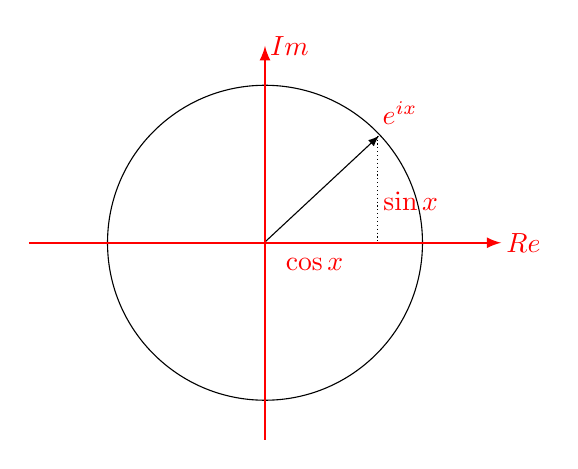
\begin{tikzpicture}
            \draw[draw=black, thin, solid] (-1.00,0.00) ellipse (2.00 and 2.00);
            \draw[draw=black, -latex, thin, solid] (-1.00,0.01) -- (0.45,1.36);
            \draw[draw=black, thin, densely dotted] (-1.00,0.00) -- (0.50,0.00);
            \draw[draw=black, thin, densely dotted] (0.43,1.36) -- (0.43,0.01);
            \draw[draw=red, -latex, thick, solid] (-4.00,0.00) -- (2.00,0.00);
            \draw[draw=red, -latex, thick, solid] (-1.00,-2.50) -- (-1.00,2.50);
            \node[red, anchor=south west] at (1.94,-0.25) {$Re$};
            \node[red, anchor=south west] at (-1.06,2.25) {$Im$};
            \node[red, anchor=south west] at (0.37,1.38) {$e^{ix}$};
            \node[red, anchor=south west] at (0.38,0.29) {$\sin x$};
            \node[red, anchor=south west] at (-0.86,-0.48) {$\cos x$};
        \end{tikzpicture}
    \end{center}
\end{thmbox}

\begin{thmbox}
    \begin{theorem}[Polar form of complex number]
        For any $a,b\in\R$, we have:
            $$z=a+bi \iff z=re^{ix}$$
        where $r=\sqrt{(a^2+b^2)},x=\tan^{-1}(\frac{b}{a})$.
    \end{theorem}
    \begin{prfbox}
        \begin{proof}
            \begin{eqnarray}
                z & = & r e^{i \theta} \nonumber\\
                  & = & r (\cos \theta + i \sin \theta)\nonumber\\
                  & = & r \cos \theta + i r \sin \theta\nonumber
              \end{eqnarray}
        \end{proof}
    \end{prfbox}
    
\end{thmbox}

\begin{thmbox}
    \begin{theorem}[*Roots of unity]
        The solution for $z^n=1,z\in\C$ is given by $U_n=\{e^{\frac{2\pi i}{n}k}, k=1,2,...,n-1\}$.
    \end{theorem}
    \begin{prfbox}
        \begin{proof}
            \begin{eqnarray}
                \left( e^{\frac{2 \pi i}{n} k} \right)^n & = & e^{2 \pi k i}\nonumber\\
                & = & \cos (2 \pi k) + i \sin (2 \pi k)\nonumber\\
                & = & \cos 0 + i \sin 0\nonumber\\
                & = & 1 \nonumber
            \end{eqnarray}
        \end{proof}
    \end{prfbox}    
\end{thmbox}


\begin{thmbox}
    \begin{theorem}[Fundamental Theorem of Algebra]
        Every non-constant polynomial over $\mathbb{C}$ has a root in $\mathbb{C}$.
    \end{theorem}
\end{thmbox}


\newpage

\setcounter{section}{3}

\section{Groups}

Before we define groups, it is necessarily for us to define binary operation.

\begin{defbox}
    \begin{definition}[Binary operation]
        A binary operation $\ast$ on a set $S$ is a map, where $\ast : S \times S \rightarrow S$ and $\ast : (a, b) \mapsto a \ast b$
    \end{definition}
\end{defbox}

For example, the addition operation $+$ is a binary operation, where $$+:\C\times\C\to\C$$

\begin{thmbox}
    \begin{proposition}
        If $|S|=n$, then there are $n^{(n^2)}$ binary operations on $S$.
    \end{proposition}
\end{thmbox}


We define a group as the following:

\begin{defbox}
    \begin{definition}[Group]
        A group is a set $G$ with a binary operation $*$ on $G$ such that the following axioms are satisfied:\\
        \begin{enumerate}
            \item There is $e\in G$, s.t. $\forall a\in G, e*a=a*e*a$ (Existance of identity element)
            \item For every $a\in G,\exists a'\in G,$ s.t. $a'*a=a*a'=e$ (Existance of inverse element)
            \item For any $a,b,c\in G, (a*b)*c=a*(b*c)$ (Associativity)
        \end{enumerate}
    \end{definition}
\end{defbox}

\begin{expbox}
    \begin{example}
        Prove that $(\R,+)$ is a group.\\

        \begin{enumerate}
            \item There is $0\in\R,0+a=a+0=a,\forall a\in\R$
            \item There is $-a\in\R,-a+a=a+(-a)=0,\forall a\in\R$
            \item Addition is associative in $\R$
        \end{enumerate}
        \begin{tabular}{ll}
            &\\
        \end{tabular}
        
        Therefore $(\R,+)$ is a group by definition.
    \end{example}
\end{expbox}

Note that $\Z,\Q,\C$ are groups under the binary operation $+$.\\\\
However, $\N$ is not a group under $+$ since there is no $a'\in\N$, s.t. $a+a'=0$.

\begin{expbox}
    \begin{example}
        Is $\R$ a group under $\cdot$?\\\\
        Since for $0\in\R$, there is no $0'$, s.t. $0'\cdot 0=1$, therefore $\R$ is not a group under $\cdot$.
    \end{example}
\end{expbox}

To solve the issue, from now on, we define $\R^*$, where $0$ is being removed from $\R$. i.e. 
$$\R^*=\R-{0}$$
We will apply this notation for other sets also, such as $\Z,\C,\Q,...$

\begin{expbox}
    \begin{example}
        Is $\C^*$ a group under multiplication?\\\\
        We start to check the three axioms:

        \begin{tabular}{ll}
            &\\
        \end{tabular}

        \begin{enumerate}
            \item There is $1\in \C^*$, s.t. $a\cdot 1=1\cdot a=a$
            \item The inverse element exists, since:
            $$\frac{1}{a+bi}=\frac{1}{a+bi}\left(\frac{a-bi}{a+bi}\right)=\frac{a-bi}{a^2+b^2}=\frac{a}{a^2+b^2}-\frac{b}{a^2+b^2}i$$
            and $(a+bi)\left( \frac{a}{a^2+b^2}-\frac{b}{a^2+b^2}i\right)=1$
            \item The operation is associative for sure.
        \end{enumerate}

        \begin{tabular}{ll}
            &\\
        \end{tabular}

        Hence $\C^*$ a group under multiplication by definition.
    \end{example}
\end{expbox}

\begin{defbox}
    \begin{definition}[Abelian groups]
        If $(G, \ast)$ is a group, and if $\ast$ is commutative $(a \ast b = b \ast a), \forall a, b \in G$, then $G$ is called abelian group.
    \end{definition}
\end{defbox}


\begin{expbox}
    \begin{example}
        Let $M_n (\mathbb{R})$ be a set of $n \times n$ matrice, with all real number entries.\\

        If $n \geq 2$, then the multiplication is not commutative and therefore not abelian.\\

        However, is $M_n (\mathbb{R})$ a group under matrix multiplication?\\

    
        Let $A \in M_n (\mathbb{R})$. Note that there is matrix with $| A | = 0$, for such matrix, There is no
        $A'$, s.t. $A A' = A' A = I$\\

        Thus $M_n (\mathbb{R})$ is not a group under matrix multiplication.
    \end{example}
\end{expbox}

Similarly, we can create a new set, where $| A | \neq 0, \forall A \in M_n
(\mathbb{R})$. Such set is called $\text{GL} (n, \mathbb{R})$.

\begin{expbox}
    \begin{example}
        \begin{example*}
            Is $\text{GL} (n, \mathbb{R})$ a group under matrix multiplication?\\
            
            We first prove that the operation is binary. We need to prove that $A \times
            B \in \text{GL} (n, \mathbb{R})$\\
            
            Note that $| A \cdot B | = | A | | B | \neq 0$. Thus the operation is closed.\\
            
            We now prove that $\text{GL} (n, \mathbb{R})$ is a group under matrix
            multiplication.\\
            \begin{enumerate}
              \item There is $I_n$, such that $I_n A = A I_n = A$\\
              
              \item As $| A | \neq 0, \forall A \in \text{GL} (n, \mathbb{R})$, thus
              there is $A^{- 1}$, s.t. $A A^{- 1} = A^{- 1} A = I$\\
              
              \item It is obvious that the multiplication of matrix is associative.\\
            \end{enumerate}
            Thus $\text{GL} (n, \mathbb{R})$ is a group under matrix multiplication.\\
            
            Note that when $n \geq 2$, the group is not Abelian.
          \end{example*}
    \end{example}
\end{expbox}

\begin{defbox}
    \begin{definition}[Finite groups]
        For a group $(G, \ast)$,\\
        \begin{itemize}
            \item The group is called finite group, if $G$ is a finite set.
            
            \item The group is called infinite group, if $G$ is a infinite set.
        \end{itemize}
    \end{definition}
\end{defbox}

\begin{expbox}
    \begin{example}
        Let $U_n = \{ z \in \mathbb{C}|z^n = 1 \}$. Consider the multiplication operation in $U_n$.\\

        We first prove the set is closed under multiplication.\\

        Pick any 2 arbitrary element from $U_n$, $z_1 \text{ and } z_2$.\\

        Note that $(z_1 \cdot z_2)^n = z_1^n \cdot z^n_2 = 1 \cdot 1 = 1 \in U_n$ (As
        $1^n = 1, \forall n \in \mathbb{N}$), hence $z_1 \cdot z_2 \in U_n$. $U_n$ is
        closed under $\cdot$. $\cdot$ is a binary operator.\\

        Now we prove that $(U_n, \cdot)$ is a group.\\

        \begin{itemize}
        \item There is an identity element $1 \in U_n$, such that $z^n \cdot 1 = 1
        \cdot z^n = z^n$\\
        
        \item If $z \in U_n$, then $\left( \frac{1}{z} \right)^n = \frac{1}{z^n} =
        \frac{1}{1} = 1 \in U_n$, thus $\forall z \in U_n, \exists \frac{1}{z^n}$,
        s.t. $z^n \left( \frac{1}{z^n} \right) = 1$\\
        
        \item Complex number are associative under multiplication.\\
        \end{itemize}
        Thus $(U_n, \cdot)$ is a group.\\

        Note that we may express $U_n = \left\{ e^{\frac{2 \pi i}{n} k} |k = 0, 1,
        \ldots, n - 1 \right\}$, hence $| U_n | = n$\\

        \hrulefill

        At the first glance, we observe that
        \begin{eqnarray*}
        z_1 \cdot z_2 & = & e^{\frac{2 \pi i}{n} k_1} \cdot e^{\frac{2 \pi i}{n}
        k_2}\\
        & = & e^{\frac{2 \pi i}{n} (k_1 + k_2)}\\
        \end{eqnarray*}

        It is possible that $k_1 + k_2 > n - 1$, however, under modulo operation,

        \[ \exists k, 0 \leq n - 1, k \equiv (k_1 + k_2) \text{ mod } n \]
    \end{example}
\end{expbox}

Now consider a mod 3 modulo group. We can partition $\Z$ into 3 groups, namely 
$$\Z=3\Z\sqcup 3\Z +1 \sqcup 3\Z +2$$
Where
\begin{eqnarray}
    3\Z & = & \{3n|n\in\Z\}\nonumber\\
    3\Z + 1 & = & \{3n + 1|n\in\Z\}\nonumber\\
    3\Z + 2 & = & \{3n + 2|n\in\Z\}\nonumber
\end{eqnarray}

If we let the operation $+$ to be the same as $+$ in $\Z$, we can make a modular 3 addition table as: 

\begin{center}
    {\center{$\begin{array}{|c|ccc|}
        \hline
        + & 0 & 1 & 2\\
        \hline
        0 & 0 & 1 & 2\\
        1 & 1 & 2 & 0\\
        2 & 2 & 0 & 1\\
        \hline
      \end{array}$}}
\end{center}

Partition $\Z$ as $$\mathbb{Z}= n\mathbb{Z} \sqcup (n\mathbb{Z}+ 1) \sqcup \cdots \sqcup
(n\mathbb{Z}+ n - 1)$$

for any integers, we have $n\Z+k=\{mn+k|m\in\Z\}$. We have the following proposition:

\begin{thmbox}
    \begin{proposition}
        $\Z_n$ is a finite, abelian group under modulo $n$ addition, and $|\Z_n|=n$
    \end{proposition}    
\end{thmbox}

The following theorem is very important throughtout the entire course!

\begin{thmbox}
    \begin{theorem}[Left and right cancellation law]
        If $(G, \ast)$ is a group, then the left cancellation and right cancellation law holds in group.\\
        \begin{itemize}
            \item Left cancellation law: $a*b=a*c\implies b=c$
            \item Right cancellation law: $a*b=c*b\implies a=c$
        \end{itemize}
    \end{theorem}
    \begin{prfbox}
        \begin{proof}
            Only left cancellation law is proved since right cancellation law can be proved similarly.
    
            \begin{eqnarray}
                a \ast b & = & a \ast c\nonumber\\
                a^{- 1} (a \ast b) & = & a^{- 1} (a \ast c)\nonumber\\
                (a^{- 1} a) \ast b & = & (a^{- 1} a) \ast c \hspace*{\fill}
                \nonumber\\
                e \ast b & = & e \ast c \hspace*{\fill} \nonumber\\
                b & = & c \hspace*{\fill}  \nonumber
              \end{eqnarray}
        \end{proof}
    \end{prfbox}
    
\end{thmbox}


\begin{warnbox}
        \begin{warning}
            Note that $a*c=b*a\centernot\implies c=b$
        \end{warning}
        \begin{prfbox}
            \begin{proof}
                Pick two element from $\text{ GL} (\mathbb{Z}, 2)$, where $A =
                \left[\begin{array}{cc}
                  1 & 1\\
                  0 & 1
                \end{array}\right], B = \left[\begin{array}{cc}
                  1 & 0\\
                  2 & 1
                \end{array}\right]$.\\
                
                (Remark: Lower triangle matrix and Upper triangle matrix do not commute)\\
                
                Define $C = A B A^{- 1} \implies C A = A B$ (By multiplying $A$ on both
                side)\\
                
                Find the inverse of $A$: (Trick)\\
                
                $\left[\begin{array}{cc}
                  1 & x\\
                  0 & 1
                \end{array}\right] \left[\begin{array}{cc}
                  1 & y\\
                  0 & 1
                \end{array}\right] = \left[\begin{array}{cc}
                  1 & x + y\\
                  0 & 1
                \end{array}\right] = \left[\begin{array}{cc}
                  1 & 0\\
                  0 & 1
                \end{array}\right]$, thus inverse $A^{- 1} = \left[\begin{array}{cc}
                  1 & - x\\
                  0 & 1
                \end{array}\right] = \left[\begin{array}{cc}
                  1 & - 1\\
                  0 & 1
                \end{array}\right]$\\
                
                As a result, we have $C = \left[\begin{array}{cc}
                  1 & 1\\
                  0 & 1
                \end{array}\right] \left[\begin{array}{cc}
                  1 & 0\\
                  2 & 1
                \end{array}\right] \left[\begin{array}{cc}
                  1 & - 1\\
                  0 & 1
                \end{array}\right] = \left[\begin{array}{cc}
                  3 & - 2\\
                  2 & - 1
                \end{array}\right] \neq \left[\begin{array}{cc}
                  1 & 0\\
                  2 & 1
                \end{array}\right]$\\
                
                Thus $C A = A B$ does not implies that $C = B$, thus $a \ast c = b \ast a
                \centernot\implies c = b$.
            \end{proof}
        \end{prfbox}
        
\end{warnbox}



\begin{thmbox}
    \begin{corollary}[Uniqueness of identity and inverse element]
        If $(G,*)$ is a group, then for any $a\in G$, the inverse element $a'$ s.t. $aa'=e$ is $\mathbf{unique}$.\\
        The identity element $e$ for each group is also unique.
    \end{corollary}
    \begin{prfbox}
        \begin{proof}
            Assume that there are two inverse element $a'$ and $a''$ in $G$, for $a\in G$. We then have:\\
            \begin{center}
                $\left\{\begin{array}{l}
                    a \ast a' = e\\
                    a \ast a'' = e
                  \end{array}\right.$    
            \end{center}
            By left cancellation law, $a'=a''$\\\\
            Similarly, assume there are two identity element $e'$ and $e''$ in $G$. We then have:\\
            \begin{center}
                $\left\{\begin{array}{l}
                    e' \ast e'' = e'\\
                    e' \ast e'' = e''
                  \end{array}\right.$
            \end{center}
            By left cancellation law, $e'=e''$
        \end{proof}
    \end{prfbox}
\end{thmbox}

\begin{expbox}
    \begin{example}[2023 Homework 1, Problem 3, Modified]
        If $(G, *)$ is a group, $a, b, c \in G$, prove that $abc = e$ implies that $bca = e$. 
    \end{example}
    \begin{prfbox}
        \begin{proof}[1]
            Since $a,b,c\in G$, by associative property of groups, we have:
            $$abc=a(bc)=e$$
            By the property of inverse element of groups, we also have:
            $$a(bc)=(bc)a=e$$
            Therefore, if $abc=e$, then $abc=(bc)a=bca=e$.              
        \end{proof}
    \end{prfbox}
    \begin{prfbox}
        \begin{proof}[2]
            Consider the element $g=a^{-1}abca$. For the associativity, we have $g=a^{-1}(abc)a=a^{-1}ea$.\\\\
            On the other hand, we have $g=(a^{-1}a)bca=bca$.\\\\
            Above all, we proved that $bca=e$.
        \end{proof}
    \end{prfbox}
\end{expbox}

\newpage

\section{Subgroups}

Before we define subgroup, we shall define the ``closeness'' of operation.

\begin{defbox}
    \begin{definition}[Closeness of operation]
        Let $T$ be a set, $*$ be a binary operation on $T$. If $S\subset T$ is a subset, then $S$ is closed under $*$ if 
        $$\forall a,b\in S, a*b\in S$$
        If $S$ is closed under $\ast$ on $T$, we can view $\ast$ as binary operation on $S$. We call such binary operation the induced operation from $\ast$ on
$T$.
    \end{definition}
\end{defbox}

Under such defintion, if we let $T =\mathbb{R}$, then $\mathbb{Z}, \mathbb{Q},
\mathbb{R}_{> 0}, \mathbb{R}_{< 0}$ are closed under +.

However, $2\mathbb{Z}+ 1$ is not closed since, $1, 3 \in 2\mathbb{Z}+ 1$, but $1 + 3 = 4 \not\in 2\mathbb{Z}+ 1$.

\begin{defbox}
    \begin{definition}[Subgroup]
        If $T$ is a set, $*$ is a binary operation on $T$.\\
        A subset $S$ in $T$ is closed under $*$ if for any $a,b\in S,$
    \end{definition}
\end{defbox}

\begin{expbox}
    \begin{example}
        $\mathbb{Z}, \mathbb{Q}$ are subgroup of $(\mathbb{R}, +)$.
    \end{example}
\end{expbox}

\begin{expbox}
    \begin{example}
        Let $S = \left\{ n|n \not\in \mathbb{Q} \text{ and } n \in \mathbb{R}
\right\}$ to be the set of real irrational numbers, then $S$ is not closed
under the addition. One counterexample will be $\pi + (- \pi) = 0 \not\in
S$.
    \end{example}
\end{expbox}

\begin{expbox}
    \begin{example}
        $\mathbb{R}_{> 0}$ is not a subgroup of $(\mathbb{R}, +)$. It is because
        it does not satisfy the group definition, as the identity element and inverse
        element does not exist.
    \end{example}
\end{expbox}

\begin{expbox}
    \begin{example}
        Let $(\mathbb{C}^{\ast}, \cdot)$ be a group. Determine whether the following are subgroups.

            {\noindent}\begin{tabularx}{1.0\textwidth}{|@{}X@{}|@{}X@{}|@{}X@{}|@{}X@{}|}
            \hline
            1. $U_2 = \{ 1, - 1 \}$ & 2. $\{ 1, 2, 2^2, 2^3, \ldots \}$ & 3. $\left\{ 1, 2,
            \frac{1}{2}, 2^2, \ldots \right\}$ & 4.$\mathbb{R}_{> 0}$\\
            
            \hline

            \end{tabularx}\\

        Only 2 is not a subgroup, since inverse element does not exist for most of the elements.\\
        (e.g. $2^{-1}=\frac{1}{2}\not\in \{1,2,2^2,2^3,...\})$
    \end{example}
\end{expbox}

\begin{expbox}
    \begin{example}
                Let $(\mathbb{C}^{\ast}, \cdot)$ be a group. Is $U = \{ z \in
        \mathbb{C}^{\ast} : | z | = 1 \}$ a subgroup? where $| z | = \sqrt{a^2 +
        b^2}$.\\\\

        We first check whether the operation is closed or not.\\

        Note that $\forall z, w \in \mathbb{C}, | z w | = | z | | w | .$ If $z, w \in
        U$, $| z w | = | z |  | w | = 1 \times 1 = 1$ and obviously, $1 \in U$.\\

        Thus we know that $U$ is closed under $\cdot$.\\

        Then we check whether the inverse element exists.\\
        \begin{eqnarray*}
        | z \cdot z' | & = & | 1 |\\
        | z |  | z' | & = & 1\\
        | z' | & = & 1 \in U
        \end{eqnarray*}\\
        Thus the inverse element exist.\\

        Finally, the multiplication of $\mathbb{C}^{\ast}$ is associative.\\

        Thus $U = \{ z \in \mathbb{C}^{\ast} : | z | = 1 \}$ is a subgroup.
    \end{example}
\end{expbox}

\begin{expbox}
    \begin{example}
        Let $\text{GL} (3, \mathbb{R})$ be a group of $3 \times 3$ real matrix under
        $\cdot$, where $| M | \neq 0, \forall M \in \text{GL} (3, \mathbb{R})$.\\

        Are the following sets a subgroup under matrix multiplication?\\
        \begin{enumerate}
        \item $A =$All $3 \times 3$ diagonal real matrix, with positive integer
        entry.\\
        
        \item $B =$All $3 \times 3$ diagonal real matrix, with $| M | = 1$\\
        
        \item $C =$All $3 \times 3$ upper triangular real matrix, $| M | \neq 0$,
        non-negative entry\\\\
        \end{enumerate}

        Before we do the question, it will be good to know some of properties.

        1. Matrix multiplication of diagonal matrix
        \[ \left[\begin{array}{ccc}
            a_1 &  & \\
            & a_2 & \\
            &  & a_3
        \end{array}\right] \times \left[\begin{array}{ccc}
            b_1 &  & \\
            & b_2 & \\
            &  & b_3
        \end{array}\right] = \left[\begin{array}{ccc}
            a_1 b_1 &  & \\
            & a_2 b_2 & \\
            &  & a_3 b_3
        \end{array}\right] \]
        2. Inverse of diagonal matrix
        \[ \left[\begin{array}{ccc}
            a_1 &  & \\
            & a_2 & \\
            &  & a_3
        \end{array}\right]^{- 1} = \left[\begin{array}{ccc}
            a^{- 1}_1 &  & \\
            & a^{- 1}_2 & \\
            &  & a^{- 1}_3
        \end{array}\right] \]\\
        Given the above properties, it will be easy for us to solve the question.\\

        \begin{enumerate}
            \item The operation is closed. However, most of the inverse does not exist. For
            example:
            \[ \left[\begin{array}{ccc}
                2 &  & \\
                & 3 & \\
                &  & 5
            \end{array}\right]^{- 1} = \left[\begin{array}{ccc}
                \frac{1}{2} &  & \\
                & \frac{1}{3} & \\
                &  & \frac{1}{5}
            \end{array}\right] \not\in A \]\\
    
            \item Yes, note that the group is also abelian.\\
            \item The operation is closed. However, most of the inverse does not exist. For
            example:
            \[ \left[\begin{array}{ccc}
                1 & 2 & \\
                & 1 & \\
                &  & 1
            \end{array}\right]^{- 1} = \left[\begin{array}{ccc}
                1 & - 2 & \\
                & 1 & \\
                &  & 1
            \end{array}\right] \not\in C \]
        \end{enumerate}
    \end{example}
\end{expbox}

\newpage 

Let $G$ be a group under $*$. Then we will be using the following set of notation throughtout the course:

\begin{eqnarray}
    a*b & = & ab \nonumber\\
    \underbrace{a*a*...*a}_{n} & = & a^n \nonumber\\
    a' & = & a^{-1} \nonumber\\
    \underbrace{a'*a'*...*a'}_{n} & = & a^{-n} \nonumber\\
    a^0 & = & e \nonumber
\end{eqnarray}

\begin{thmbox}
    \begin{theorem}[*Subgroup]
        A subset $H$ of group $G$ is a subgroup if and only if\\
        \begin{enumerate}
            \item $H$ is closed under binary operation of $G$\\
            \item The identity element in $G: e\in H$\\
            \item For any $a\in H$, $a^{-1}\in H$\\
        \end{enumerate}
    \end{theorem}
    \begin{prfbox}
        \begin{proof}
            $(\implies)$\\\\
            If $H$ is a subgroup, by the definition of subgroup, $H$ is closed under
            binary operation of $G$.\\
    
            $H$ is a group under reduced operation, thus there is $e'$, which is the
            identity element of $H$. \\
            
            We now prove that $e' = e$, where $e$ is the identity element of $G$.\\
    
            \[ \left\{\begin{array}{l}
                e' e' = e'\\
                e' e = e'
            \end{array}\right. \implies e' e' = e' e \implies e' = e \]\\
    
            by the left cancellation law.\\
    
            Finally it is obvious that the associativity holds.\\
    
            $(\Longleftarrow)$\\\\
            If the three rules holds, then we have:\\
    
            \begin{itemize}
                \item $H$ is closed\\
                \item Identity element $e$ exists in $H$\\
                \item For every $a\in H,\exists a^{-1}\in H$\\
                \item Associativity holds
            \end{itemize}
    
        \end{proof}
    \end{prfbox}
    
\end{thmbox}

\newpage

\section{Cyclic Groups}

\begin{thmbox}
    \begin{proposition}
        Let $G$ be a group and let $a \in G$. The set $\langle a \rangle = \{ a^n : n \in \mathbb{Z} \}$ is a subgroup of $G.$\\\\
        Moreover, $\langle a \rangle$ is the smallest subgroup. i.e. if $H$ is a subgroup, $a \in H$, then $\langle a \rangle \subset H$.
    \end{proposition}
    \begin{prfbox}
        \begin{proof}
            Since that $a^m a^n = a^{m + n} \in H$, the operation is therefore closed.\\
    
            The identity element $e$ exists in $\langle a \rangle$ because if we pick $n = 0$, then
            $a^0 = e$.\\
    
            The inverse element $a' = a^{- n}$ also exists in $\langle a \rangle$.\\
    
            Thus $\langle a \rangle$ is the smallest subgroup.
        \end{proof}
    \end{prfbox}    
\end{thmbox}

\begin{warnbox}
    \begin{warning}
        Be reminded that $a^n$ implies $n$ copies of \textbf{binary operation, not
        power}.
    \end{warning}
\end{warnbox}


\begin{expbox}
    \begin{example}
        For the group $(\C^*,*)$, we have
        \begin{eqnarray} 
            \langle 2 \rangle & = & \{ 2^n : n \in \mathbb{Z} \} = \left\{ 1, 2, \frac{1}{2}, 4, \frac{1}{4}, \ldots \right\} \nonumber\\
            \cyclic{-1} & = & \{(-1)^n\}=\{-1,1\} \nonumber\\
            \cyclic{i}  & = & \{(i)^n\} = \{i,1,-i,-1\} \nonumber
        \end{eqnarray}
    \end{example}
\end{expbox}

Note that $\cyclic{n}$ is infinite for any $n\in\Z$ except 0 since $\cyclic{0}=\{0\}$.

\begin{defbox}
    \begin{definition}[Cyclic group]
        A group $G$ is called a cyclic group if there is a special element $a\in G$, s.t. $\cyclic{a}=G$.\\\\
        We call $a$ as the generator of $G$.
    \end{definition}
\end{defbox}

\begin{expbox}
    \begin{example}
        $(\Z,+)$ is a cyclic group since $1,-1$ can generate $\Z$.
    \end{example}
\end{expbox}

\begin{expbox}
    \begin{example}
        $(\Z_n,+)$ is a cyclic group since $1$ can generate $\Z_n$.
    \end{example}
\end{expbox}

\begin{expbox}
    \begin{example}
        \nline\\
        $(U_n, \cdot) = \left\{ e^{\frac{2 \pi i}{n} k} : k = 0, 1, 2, \ldots, \right\}$ is a cyclic group as $e^{\frac{2 \pi i}{n}}$ can generate $U_n$.
    \end{example}
\end{expbox}

\newpage

\begin{expbox}
    \begin{example}
        $(\mathbb{Q}^{\ast}, +)$ is not cyclic.
    \end{example}
    \begin{prfbox}
        \begin{proof}
            Suppose the group is cyclic, then there is $ a \in \mathbb{Q}$, s.t. $\cyclic{a} = \{ n a : n \in \mathbb{Z} \} =\mathbb{Q}$.\\
    
            Since $a$ is rational, therefore $a = \frac{p}{q}, (p, q) \in \mathbb{Z} \times \{\mathbb{Z} \backslash \{ 0,1 \}\}$.\\
    
            Then we may write $\frac{1}{q^2} = n a = n \frac{p}{q} \Rightarrow \frac{1}{q} = n p \in \mathbb{Z}$, but $\frac{1}{q} \nin \mathbb{Z}$, contradiction!
        \end{proof}
    \end{prfbox}
    
\end{expbox}



\begin{expbox}
    \begin{example}
        $(\mathbb{Q}^{\ast}, *)$ is not cyclic.
    \end{example}
    \begin{prfbox}
        \begin{proof}
            If $\cyclic{a} =\mathbb{Q}^{\ast}$, then $a = \frac{p}{q} = p^{k_1}_1 \ldots .p^{k_n}_n \infixor - p^{k_1}_1 \ldots .p^{k_n}_n$, where $p_1, \ldots, p_n$ are distinct primes.\\
    
            For example, we can express $\frac{10}{77} = 2 \times 5 \times 7^{- 1} \times 11^{- 1}$.\\
    
            Let $p \nin \{ p_1, \ldots, p_n \}$,then $p \nin \cyclic{a}$, however $p \in \mathbb{Z} \in \mathbb{Q}^{\ast}$, contradiction!
        \end{proof}
    \end{prfbox}
    
\end{expbox}



\begin{expbox}
    \begin{example}
        $(\mathbb{R}, +)$ is not cyclic.
    \end{example}
    \begin{prfbox}
        \begin{proof}
            For any $a\neq 0$, $\frac{1}{2}a \nin \cyclic{a}$, contradiction!
        \end{proof}
    \end{prfbox}
    
\end{expbox}



\begin{expbox}
    \begin{example}
        \nline\\
        Let $S = \left\{ \left[\begin{array}{cc}
            1 & n\\
            0 & 1
          \end{array}\right] : n \in \mathbb{Z}_{\geqslant 1} \right\}$. Then $G = (S,
          \times)$ is cyclic.
    \end{example}
    \begin{prfbox}
        \begin{proof}
            \nline\\
            Let $a = \left[\begin{array}{cc}
                1 & 1\\
                0 & 1
              \end{array}\right]$. Observe that $\left[\begin{array}{cc}
                1 & 1\\
                0 & 1
              \end{array}\right]^n = \left[\begin{array}{cc}
                1 & n\\
                0 & 1
              \end{array}\right]$.
        \end{proof}
    \end{prfbox}
\end{expbox}




\newpage

\begin{thmbox}
    \begin{theorem}
        Any cyclic group $G$ is abelian.
    \end{theorem}
    \begin{prfbox}
        \begin{proof}
            If $G$ is cyclic, then $G=\cyclic{a}=\{a^n:n\in\Z\}$.\\\\
            Pick any element $x,y\in G$, where $x=a^m,y=a^n$. We have:
            \begin{eqnarray*}
                xy & = & a^ma^n\\
                   & = & a^{m+n}\\
                   & = & a^na^m\\
                   & = & yx
            \end{eqnarray*}
        \end{proof}
    \end{prfbox}    
\end{thmbox}


\begin{thmbox}
    \begin{theorem}
        If $\cyclic{a}$ is infinite, then for any $n\in\N, a^n \neq e$.
    \end{theorem}
    \begin{prfbox}
        \begin{proof}
            Assume that $a^n=e$ for some $n$, and assume that $n$ is the smallest such exponential.\\
            Then $\{e,a,a^2,...,a^n\}$ already forms a subgroup. This contradicts the fact that $\cyclic{a}$ is infinite.
        \end{proof}
    \end{prfbox}    
\end{thmbox}


\begin{defbox}
    \begin{definition}[Order]
        If $a^n\neq e$ for any $n\in\N$, we call $a$ has infinite order, or has order $\infty$.\\
        If $a^n=e$ for some positive integer $n$, then the smallest positive integer $n$ is called the order of $a$.
    \end{definition}
\end{defbox}

\begin{expbox}
    \begin{example}
        Let $G=(\R,+)$. Then any $a\in\R-{0}$ has order $\infty$.
    \end{example}

    \begin{prfbox}
        \begin{proof}
            If $a=0$, then then $a^n = \underset{n}{\underbrace{a + a + a + \cdots + a}} = n a \neq 0$.\\\\
            If $a=0$, then a is already the identity element and the order is thus 1.\\\\
            In fact, for any group $G$, if $e\in G$ is the identity element, we always have $\ord{e}=1$. 
        \end{proof}
    \end{prfbox}
    
\end{expbox}



\begin{expbox}
    \begin{example}
        Let $G=C^*$, then:
        \begin{eqnarray*}
            \ord{2} & = & \infty \\
            \ord{-1} & = & 2\\
            \ord{i} & = & 4\\
            \ord{1} & = & 1\\
        \end{eqnarray*}
    \end{example}
\end{expbox}

\begin{expbox}
    \begin{example}
        Let $G=(\Z_12,+)$. We have:
        
        \begin{eqnarray*}
            \cyclic{3} =  \{3,6,9,12\to 0\}\implies\ord{3}&=&4\\
            \cyclic{5} =  \{5,...,60\to 0\}\implies\ord{5}&=&12\\
            \cyclic{8} =  \{3,6,9,12\to 0\}\implies\ord{3}&=&4
        \end{eqnarray*}
    \end{example}
\end{expbox}

To help us to prove further results about groups, we shall introduce the division algorithm for $\Z$.

Intuitively, consider $n \div m, n \in \mathbb{Z}, m \in \mathbb{Z}_{> 0}$, we always get quotient and remainder $0 \leqslant r < m$. We then have the following theorem:

\begin{thmbox}
    \begin{theorem}[Division algorithm for $\Z$]
        If $m\in\Z_{>0}$ and $n\in\Z$, then there exist unique integers $q,r$, s.t.
        $$n=mq+r \infixand   0\leq r < m$$
    \end{theorem}
\end{thmbox}

With the above theorem, we can prove the following theorem:

\begin{thmbox}
    \begin{theorem}
        If $G$ is a cyclic subgroup, then every subgroup of $G$ is also cyclic.
    \end{theorem}
    \begin{prfbox}
        \begin{proof}
            Let $G=\cyclic{a}$. Let $H\subset G$ be a nonempty subgroup.\\\\
            If $H=\{e\}$, then $\cyclic{e}=\{e\}$, which proves that $H$ is cyclic.\\\\
            If $H\neq\{e\}$, then there is $b\in H$, such that 
            $\left\{\begin{array}{lll}
                b & = & a^k\\
                b^{- 1} & = & a^{- k}
              \end{array}\right., b, b^{- 1} \in H$.\\
    
              As one of the $k, - k$ must be greater than 0, therefore there
              exist $n \in \mathbb{Z}_{> 0}$, s.t. $a^n \in H$.\\
              
              Let $S = \{ n \in \mathbb{Z}_{> 0} : a^n \in H \}$, then $S$ is not empty.\\
              
              Let $m$ be the smallest element in $S$. We claim $H = \cyclic{a^{nm}}.$\\
              
              As $a^m \in H$, $\cyclic{a^m} \subset H$.\\
              
              For $b \in H$, since $b \in G = \cyclic{a}$, therefore $b = a^n$ for some $n \in \mathbb{Z}.$\\
              
              Consider $n \div m$. By division algorithm\\
              \begin{eqnarray*}
                n & = & m q + r\\
                r & = & n - m q
              \end{eqnarray*}
              \[ a^r = a^{n - m q} = a^n a^{- m q} = a^n (a^m)^{- q} \in H \]\\
              Note that $a^r \in H$, and $m$ was the smallest positive integer s.t. $a^m \in
              H$, hence $r = 0$.\\
              
              Thus $b = a^n = (a^m)^q \in \cyclic{a^n}$, $H \subset \cyclic{a^m}$, thus $H = \cyclic{a^m}$
        \end{proof}
    \end{prfbox}
    
\end{thmbox}


\begin{thmbox}
    \begin{corollary}
        Every subgroup of $\Z$ is $n\Z$ for some $n\in\Z$.
    \end{corollary}
    \begin{prfbox}
        \begin{proof}
            As $\mathbb{Z}$ is cyclic, thus $H = \cyclic{n} = n\mathbb{Z}$.\\
    
            For $s, r \in \mathbb{Z} \infixand s, r \neq 0$, define $H = \{ m s + n r : m,n \in \mathbb{Z} \}$.\\\\
            Then $H$ is closed. ($\because (m_1 s + n_1 r) + (m_2 s + n_2 r) = (m_1 + m_2) s + (n_1 + n_2) r
            \in H$)\\
    
            Note that the identity element 0 also exists as $0 s + 0 r = 0 \in H$.\\
    
            If $(m s + n r) \in H, \text{ then } - (m s + n r) \in H$. Now $H$ is a
            subgroup of $\mathbb{Z}$, thus $H = d\mathbb{Z}$ for some $d \in \mathbb{Z}$.\\
    
            Consider the properties of $d$:\\
            \begin{itemize}
            \item $d$ is a positive integer.\\
            
            \item $s \in H \subset d\mathbb{Z}$ implies $d$ is a divisor of s and $d$ is
            a divisor of $r$. Hence $d$ is a common divisor of $s$ and $r$.\\
            
            \item Let $d'$ to be another common divisor of \ $s \infixand r$. $d'$ is
            also a divisor of every elements in $H$. In particular, $d'$ is a divisor of $d$.\\
            \end{itemize}
            From above property, we conclude $d = \text{gcd} (r, s) = m s + n r$ for
            some $n, m \in \mathbb{Z}$.
        \end{proof}
    \end{prfbox}
\end{thmbox}

\begin{thmbox}
    \begin{theorem}[*Conditions for relatively prime]
        Two integers $r,s$ are relatively prime, i.e. $\text{gcd}(r,s)=1$, if and only if there exists integer $m,n$, such that:
        $$mr+ns=1$$
    \end{theorem}
\end{thmbox}

\begin{thmbox}
    \begin{theorem}[Estimation of growth of $\Pi(n)$ (Not in syllabus)]
        Let $\Pi (n)$ to be the number of prime numbers, which are less or equal to $n$.\\
        
        We have
        \[ \lim_{n \rightarrow \infty} \frac{\Pi (n)}{\frac{n}{\ln n}} = 1 \]

        i.e. $\Pi (n) \sim \frac{n}{\ln n}$.
    \end{theorem}
\end{thmbox}

\begin{thmbox}
    \begin{theorem}
        If $H_1,H_2$ are subgroups of $G$, then $H_1\cap H_2$ is also a subgroup of $G$. 
    \end{theorem}
    \begin{prfbox}
        \begin{proof}
            Since every subgroup has an identity element $e$, thus $e\in H_1\cap H_2$.\\
            For any element $g,h$ in $G$, we have:
            \begin{eqnarray*}
                g,h\in H_1\cap H_2 & \implies & g,h\in H_1 \infixand g,h\in H_2 \\ 
                                   & \implies & gh^{-1}\in H_1 \infixand gh^{-1}\in H_2\\
                                   & \implies & gh^{-1}\in H_1\cap H_2
            \end{eqnarray*}
        \end{proof}
    \end{prfbox}
\end{thmbox}

\begin{thmbox}
    \begin{corollary}
        Let $m,n$ be non-zero integers. Then $m\Z\cap n\Z=N\Z$ for some positive integer $N$.\\

        Moreover, $N$ is a common multiple of $m,n$.
    \end{corollary}    
\end{thmbox}

\begin{thmbox}
    \begin{theorem}
        The order of $a$ is the number of elements in $\cyclic{a}$.
    \end{theorem}    
    \begin{prfbox}
        \begin{proof}
            If order of $a$ is finite, then there exists $n \in \mathbb{Z}_{> 0}$, $a^n = e, a^j \neq
            e$, $1 \leq j < n$.\\

            Then $\cyclic{a} = \{ e, a, a^2, a^3, \ldots, a^{n - 1}, a^n = e, \ldots, \}$\\

            Therefore $\cyclic{a}$ has $n$ elements.\\

            Suppose there are non-distinct elements in the set, then $a^j = a^i
            \implies e = a^{j - i}$ which leads to contradiction as we have for any $j
            < n, a^j \neq e$.\\

            If the order of $a$ is infinite, then
            \[ \cyclic{a} = \{ e, a, a^2, \ldots \} \]
            Suppose that there are non-distinct elements in the set, then $a^j = a^i
            \Rightarrow e = a^{j - i}$ which leads to contradiction as we have for any $j
            < n, a^j \neq e$.
        \end{proof}
    \end{prfbox}
\end{thmbox}

\begin{expbox}
    \begin{example}
        Consider a group $\text{GL} (2, \mathbb{R})$, compute the order of the
        following element.
        \[ a = \left[\begin{array}{cc}
            0 & 1\\
            - 1 & 0
        \end{array}\right], b = \left[\begin{array}{cc}
            1 & 0\\
            2 & 1
        \end{array}\right], c = \left[\begin{array}{cc}
            \cos \left( \frac{\pi}{101} \right) & - \sin \left( \frac{\pi}{101}
            \right)\\
            \sin \left( \frac{\pi}{101} \right) & \cos \left( \frac{\pi}{101} \right)
        \end{array}\right] \]\\\\
        Note that $a^2 = \left[\begin{array}{cc}
        0 & 1\\
        - 1 & 0
        \end{array}\right] \left[\begin{array}{cc}
        0 & 1\\
        - 1 & 0
        \end{array}\right] = \left[\begin{array}{cc}
        - 1 & 0\\
        0 & - 1
        \end{array}\right]$, we deduce that $(a^2)^2 = a^4 = I$, but still we
        need to check $a^3$. $a^3 = \left[\begin{array}{cc}
        - 1 & 0\\
        0 & - 1
        \end{array}\right] \left[\begin{array}{cc}
        0 & 1\\
        - 1 & 0
        \end{array}\right] = \left[\begin{array}{cc}
        0 & 1\\
        - 1 & 0
        \end{array}\right]$. The order of $a$ is $4$.\\\\

        For $b,$ note that $b^2 = \left[\begin{array}{cc}
        1 & 0\\
        2 & 1
        \end{array}\right] \left[\begin{array}{cc}
        1 & 0\\
        2 & 1
        \end{array}\right] = \left[\begin{array}{cc}
        1 & 0\\
        4 & 1
        \end{array}\right], b^3 = \left[\begin{array}{cc}
        1 & 0\\
        6 & 1
        \end{array}\right]$, by observation, we have $b^n =
        \left[\begin{array}{cc}
        1 & 0\\
        2 n & 1
        \end{array}\right] \neq I$.
        The order of $b$ is therefore $\infty$.\\\\

        For $c$, since for any rotational matrix, we
        have
        \[ A^n_{\theta} = \left[\begin{array}{cc}
            \cos n \theta & - \sin n \theta\\
            \sin n \theta & \cos n \theta
        \end{array}\right] \]
        As a result, we have
        \[ c^{202} = I \]
        Thus the order of $c$ is 202.
    \end{example}
\end{expbox}

\begin{expbox}
    \begin{example}
        Let $G$ be a group. $a\in G$ has order $n$. Suppose $a^m=e,m\in\Z$, prove that $m=nk,k\in\Z$.
    \end{example}    
    \begin{prfbox}
        \begin{proof}
            We write $m=nq+r$ for some $0\leq r < n$, then $r=m-nq$. Therefore, 
            \begin{eqnarray*}
                a^r & = & a^{m-nq}\\
                    & = & a^ma^{-nq}\\
                    & = & a^m(a^n)^{-q}\\
                    & = & ee^{-q}\\
                    & = & e
            \end{eqnarray*}
            Therefore $r$ must be equals to $0$. Thus $m=nq$.
        \end{proof}
    \end{prfbox}
\end{expbox}

\begin{expbox}
    \begin{example}
        Let $G$ be a group, $a,b\in G$. Prove that $ab$ and $ba$ have the same order.
    \end{example}
    \begin{prfbox}
        \begin{proof}
            Suppose $n$ is a natural number. $(ab)^n=e$ implies $\underbrace{(ab)(ab)...(ab)}_{n}=e$. 
            \begin{eqnarray*}
                (ab)(ab)...(ab) & = & e\\
               b(ab)(ab)...(ab) & = & be\\
               (ba)(ba)...(ba)b & = & eb\\
                (ba)(ba)...(ba) & = & e
            \end{eqnarray*}
            Similarly, we can prove $(ba)^n=e$ implies $(ab)^n=e$.
        \end{proof}
    \end{prfbox}
\end{expbox}

\begin{expbox}
    \begin{example}
        Suppose $G$ is finite. $a \in G$, prove that $\exists n \in \mathbb{Z}_{> 0}$, $a^n = e$.
    \end{example}
    \begin{prfbox}
        \begin{proof}
            Assume that $| G | = N$, then  \{$a, a^2, a^3, \ldots, a^N, a^{N + 1}$\}  have
        $N + 1$ element . Then there exists 2 element which are not unique from the
        piegonhole principle. Let $a^i \infixand a^j$ be such element, where $i < j$.
        Then by cancellation law we have $a^{j - i} = e$.
        \end{proof}
    \end{prfbox}
\end{expbox}

Now we state a lemma which will be useful for the proofs after (And also in exams and homework).

\begin{thmbox}
    \begin{lemma}
        Suppose $G$ is finite group, $| G | = n$, $G = \{ a_1, a_2, \ldots, a_n \}$.
        For $a \in G$, $\{ a a_1, a a_2, \ldots, a a_n \}$ is a distinct list.
    \end{lemma}
    \begin{prfbox}
        \begin{proof}
            Assume that two terms in the list are equal. By cancellation law:
            $$aa_i=aa_j\implies a_i=a_j$$
            Then $\{ a a_1, a a_2, \ldots, a a_n \}$ is simply a permutation of $G$.
        \end{proof}
    \end{prfbox}
\end{thmbox}

\begin{expbox}
    \begin{example}
        If $G$ is abelian, $| G | = n$, prove that for any $a \in G$, we have $a^n =e$.
    \end{example}
    \begin{prfbox}
        
    \begin{proof}
        We list out the element $G=\{a_1,...,a_n\}$. Then $aa_1,aa_2,...,aa_n$ is a permutation of the list.
        As $G$ is abelian, therefore:
        \begin{eqnarray*}
            a_1,...,a_n & = & aa_,aa_2,...,aa_n\\
            a^na_1,...,a^na_n & = & a_1,...,a_n\\
            a^n & = & e
        \end{eqnarray*}
    \end{proof} 
\end{prfbox}
\end{expbox}

\begin{expbox}
    \begin{example}
        Let $G={e,a,b}$ be a group. We can write a table on binary operation:
        \begin{center}
            {\center{$\begin{array}{|cccc|}
                \hline
                \ast & e & a & b\\
                e & e & a & b\\
                a & a & b & e\\
                b & b & e & a\\
                \hline
              \end{array}$}}
        \end{center}
        Note that the table is of permutation, and only hold for 2 and 3 element group.
    \end{example}
\end{expbox}

\begin{expbox}
    \begin{example}[Braid Groups]
        Let $B_3$ be a braid group with 3 strings. Define $\sigma \infixand \tau$ to be the following.
    \end{example}
\begin{center}
    \begin{tabular}{l|l}
        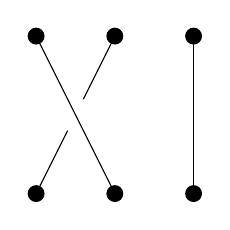
\begin{tikzpicture}
            \draw[draw=black, fill=black, thin, solid] (-1.00,2.00) circle (0.1);
            \draw[draw=black, fill=black, thin, solid] (0.00,2.00) circle (0.1);
            \draw[draw=black, fill=black, thin, solid] (-1.00,0.00) circle (0.1);
            \draw[draw=black, fill=black, thin, solid] (0.00,0.00) circle (0.1);
            \draw[draw=black, fill=black, thin, solid] (1.00,2.00) circle (0.1);
            \draw[draw=black, fill=black, thin, solid] (1.00,0.00) circle (0.1);
            \draw[draw=black, thin, solid] (1.00,2.00) -- (1.00,0.00);
            \draw[draw=black, thin, solid] (-1.00,2.00) -- (0.00,0.00);
            \draw[draw=black, thin, solid] (0.00,2.00) -- (-0.4,1.2);
            \draw[draw=black, thin, solid] (-1.00,0.00) -- (-0.6,0.8);
        \end{tikzpicture}
        &
        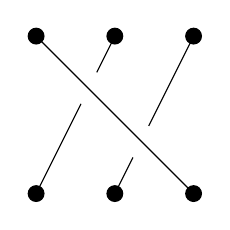
\begin{tikzpicture}
            \draw[draw=black, fill=black, thin, solid] (-1.00,2.00) circle (0.1);
            \draw[draw=black, fill=black, thin, solid] (0.00,2.00) circle (0.1);
            \draw[draw=black, fill=black, thin, solid] (-1.00,0.00) circle (0.1);
            \draw[draw=black, fill=black, thin, solid] (0.00,0.00) circle (0.1);
            \draw[draw=black, fill=black, thin, solid] (1.00,2.00) circle (0.1);
            \draw[draw=black, fill=black, thin, solid] (1.00,0.00) circle (0.1);

            \draw[draw=black, thin, solid] (-1,2) -- (1,0);
            \draw[draw=black, thin, solid] (-1,0) -- (-0.43,1.14);
            \draw[draw=black, thin, solid] (0,2) -- (-0.23,1.54);
            \draw[draw=black, thin, solid] (0,0) -- (0.23,0.46);
            \draw[draw=black, thin, solid] (1,2) -- (0.43,0.86);

        \end{tikzpicture}\\
        $\sigma$ & $\tau$\\
    \end{tabular}
\end{center}
\nline

One may define the multiplication, $\sigma \ast \tau$, by joining the graph together with $\sigma$'s bottom and $\tau$'s top. For example, $\sigma \ast\tau$ will be:

\begin{center}
\begin{tabular}{l}
    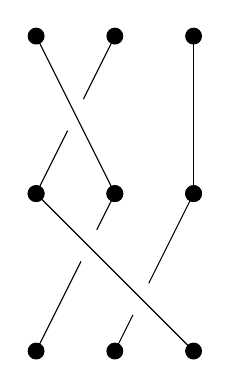
\begin{tikzpicture}
        \draw[draw=black, fill=black, thin, solid] (-1.00,2.00) circle (0.1);
        \draw[draw=black, fill=black, thin, solid] (0.00,2.00) circle (0.1);
        \draw[draw=black, fill=black, thin, solid] (-1.00,0.00) circle (0.1);
        \draw[draw=black, fill=black, thin, solid] (0.00,0.00) circle (0.1);
        \draw[draw=black, fill=black, thin, solid] (1.00,2.00) circle (0.1);
        \draw[draw=black, fill=black, thin, solid] (1.00,0.00) circle (0.1);

        \draw[draw=black, fill=black, thin, solid] (-1.00,0.00) circle (0.1);
        \draw[draw=black, fill=black, thin, solid] (0.00,0.00) circle (0.1);
        \draw[draw=black, fill=black, thin, solid] (-1.00,-2.00) circle (0.1);
        \draw[draw=black, fill=black, thin, solid] (0.00,-2.00) circle (0.1);
        \draw[draw=black, fill=black, thin, solid] (1.00,0.00) circle (0.1);
        \draw[draw=black, fill=black, thin, solid] (1.00,-2.00) circle (0.1);
        
        \draw[draw=black, thin, solid] (1.00,2.00) -- (1.00,0.00);
        \draw[draw=black, thin, solid] (-1.00,2.00) -- (0.00,0.00);
        \draw[draw=black, thin, solid] (0.00,2.00) -- (-0.4,1.2);
        \draw[draw=black, thin, solid] (-1.00,0.00) -- (-0.6,0.8);

        \draw[draw=black, thin, solid] (-1,0) -- (1,-2);
        \draw[draw=black, thin, solid] (-1,-2) -- (-0.43,-0.86);
        \draw[draw=black, thin, solid] (0,0) -- (-0.23,-0.46);
        \draw[draw=black, thin, solid] (0,-2) -- (0.23,-1.54);
        \draw[draw=black, thin, solid] (1,0) -- (0.43,-1.14);
    \end{tikzpicture}\\
    $\sigma * \tau$
\end{tabular}

\end{center}

The identity element $e$ is defined as: 

\begin{center}
    \begin{tabular}{l}
        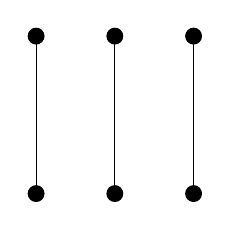
\begin{tikzpicture}
            \draw[draw=black, fill=black, thin, solid] (-1.00,2.00) circle (0.1);
            \draw[draw=black, fill=black, thin, solid] (0.00,2.00) circle (0.1);
            \draw[draw=black, fill=black, thin, solid] (-1.00,0.00) circle (0.1);
            \draw[draw=black, fill=black, thin, solid] (0.00,0.00) circle (0.1);
            \draw[draw=black, fill=black, thin, solid] (1.00,2.00) circle (0.1);
            \draw[draw=black, fill=black, thin, solid] (1.00,0.00) circle (0.1);
    
            \draw[draw=black, thin, solid] (-1,2) -- (-1,0);
            \draw[draw=black, thin, solid] (1,2) -- (1,0);
            \draw[draw=black, thin, solid] (0,0) -- (0,2);
        \end{tikzpicture}\\
        $e$
    \end{tabular}
\end{center}
\end{expbox}

\begin{expbox}
    The inverse of $\sigma$ is given by:
\begin{center}
    \begin{tabular}{l}
        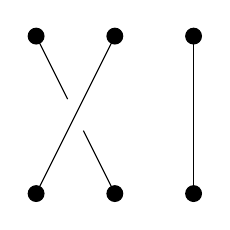
\begin{tikzpicture}
            \draw[draw=black, fill=black, thin, solid] (-1.00,2.00) circle (0.1);
            \draw[draw=black, fill=black, thin, solid] (0.00,2.00) circle (0.1);
            \draw[draw=black, fill=black, thin, solid] (-1.00,0.00) circle (0.1);
            \draw[draw=black, fill=black, thin, solid] (0.00,0.00) circle (0.1);
            \draw[draw=black, fill=black, thin, solid] (1.00,2.00) circle (0.1);
            \draw[draw=black, fill=black, thin, solid] (1.00,0.00) circle (0.1);
            \draw[draw=black, thin, solid] (1.00,2.00) -- (1.00,0.00);
            \draw[draw=black, thin, solid] (0.00,2.00) -- (-1.00,0.00);            
            \draw[draw=black, thin, solid] (-1.00,2.00) -- (-0.6,1.2);
            \draw[draw=black, thin, solid] (0.00,0.00) -- (-0.4,0.80);
        \end{tikzpicture}\\
        $\sigma^{-1}$    
    \end{tabular}
\end{center}
To see the reason, consider $\sigma * \sigma^{-1}$:
\begin{center}
    \begin{tabular}{l}
        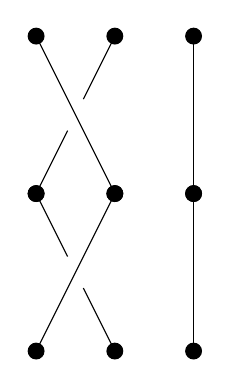
\begin{tikzpicture}
            \draw[draw=black, fill=black, thin, solid] (-1.00,2.00) circle (0.1);
            \draw[draw=black, fill=black, thin, solid] (0.00,2.00) circle (0.1);
            \draw[draw=black, fill=black, thin, solid] (-1.00,0.00) circle (0.1);
            \draw[draw=black, fill=black, thin, solid] (0.00,0.00) circle (0.1);
            \draw[draw=black, fill=black, thin, solid] (1.00,2.00) circle (0.1);
            \draw[draw=black, fill=black, thin, solid] (1.00,0.00) circle (0.1);
            \draw[draw=black, thin, solid] (1.00,2.00) -- (1.00,0.00);
            \draw[draw=black, thin, solid] (-1.00,2.00) -- (0.00,0.00);
            \draw[draw=black, thin, solid] (0.00,2.00) -- (-0.4,1.2);
            \draw[draw=black, thin, solid] (-1.00,0.00) -- (-0.6,0.8);

            \draw[draw=black, fill=black, thin, solid] (-1.00,0.00) circle (0.1);
            \draw[draw=black, fill=black, thin, solid] (0.00,0.00) circle (0.1);
            \draw[draw=black, fill=black, thin, solid] (-1.00,-2.00) circle (0.1);
            \draw[draw=black, fill=black, thin, solid] (0.00,-2.00) circle (0.1);
            \draw[draw=black, fill=black, thin, solid] (1.00,0.00) circle (0.1);
            \draw[draw=black, fill=black, thin, solid] (1.00,-2.00) circle (0.1);
            \draw[draw=black, thin, solid] (1.00,0.00) -- (1.00,-2.00);
            \draw[draw=black, thin, solid] (0.00,0.00) -- (-1.00,-2.00);            
            \draw[draw=black, thin, solid] (-1.00,0.00) -- (-0.6,-0.8);
            \draw[draw=black, thin, solid] (0.00,-2.00) -- (-0.4,-1.2);

        \end{tikzpicture}
        $\sigma * \sigma^{-1}$
    \end{tabular}
\end{center}
and then when you try to move the two strings, they will become the identity element.\\\\
In fact every braid can be represented with 4 types of elements only, and each element has inverse, thus in general every braid has inverse under such ``Multiplication''.
\end{expbox}

\setcounter{section}{7}
\newpage
\section{Groups of Permutations}
\begin{defbox}
    \begin{definition}[Permutation]
        Let $A$ be a nonempty set. A map $\phi : A \rightarrow A$ is called a permutation of A, if it is one to one and onto.
    \end{definition}
\end{defbox}



\end{document}